%%%%%%%%%%%%%%%%%%%%%%%%%%%%%%%%%%%%%%%
% Wenneker Resume/CV
% LaTeX Template
% Version 1.1 (19/6/2016)
%
% This template has been downloaded from:
% http://www.LaTeXTemplates.com
%
% Original author:
% Frits Wenneker (http://www.howtotex.com) with extensive modifications by 
% Vel (vel@LaTeXTemplates.com)
%
% License:
% CC BY-NC-SA 3.0 (http://creativecommons.org/licenses/by-nc-sa/3.0/
%
%%%%%%%%%%%%%%%%%%%%%%%%%%%%%%%%%%%%%%

%----------------------------------------------------------------------------------------
%	PACKAGES AND OTHER DOCUMENT CONFIGURATIONS
%----------------------------------------------------------------------------------------

\documentclass[a4paper,12pt]{memoir} % Font and paper size

%%%%%%%%%%%%%%%%%%%%%%%%%%%%%%%%%%%%%%%%%
% Wenneker Resume/CV
% Structure Specification File
% Version 1.1 (19/6/2016)
%
% This file has been downloaded from:
% http://www.LaTeXTemplates.com
%
% Original author:
% Frits Wenneker (http://www.howtotex.com) with extensive modifications by 
% Vel (vel@latextemplates.com)
%
% License:
% CC BY-NC-SA 3.0 (http://creativecommons.org/licenses/by-nc-sa/3.0/)
%
%%%%%%%%%%%%%%%%%%%%%%%%%%%%%%%%%%%%%%%%%

%----------------------------------------------------------------------------------------
%	PACKAGES AND OTHER DOCUMENT CONFIGURATIONS
%----------------------------------------------------------------------------------------

\usepackage{XCharter} % Use the Bitstream Charter font
\usepackage[utf8]{inputenc} % Required for inputting international characters
\usepackage[T1]{fontenc} % Output font encoding for international characters

\usepackage[top=1cm,left=1cm,right=1cm,bottom=1cm]{geometry} % Modify margins

\usepackage{graphicx} % Required for figures

\usepackage{flowfram} % Required for the multi-column layout

\usepackage{url} % URLs

\usepackage[usenames,dvipsnames]{xcolor} % Required for custom colours

\usepackage{tikz} % Required for the horizontal rule

\usepackage{enumitem} % Required for modifying lists
\setlist{noitemsep,nolistsep} % Remove spacing within and around lists

\setlength{\columnsep}{\baselineskip} % Set the spacing between columns

% Define the left frame (sidebar)
\newflowframe{0.2\textwidth}{\textheight}{0pt}{0pt}[left]
\newlength{\LeftMainSep}
\setlength{\LeftMainSep}{0.2\textwidth}
\addtolength{\LeftMainSep}{1\columnsep}
 
% Small static frame for the vertical line
\newstaticframe{1.5pt}{\textheight}{\LeftMainSep}{0pt}
 
% Content of the static frame with the vertical line
\begin{staticcontents}{1}
\hfill
\tikz{\draw[loosely dotted,color=RoyalBlue,line width=1.5pt,yshift=0](0,0) -- (0,\textheight);}
\hfill\mbox{}
\end{staticcontents}
 
% Define the right frame (main body)
\addtolength{\LeftMainSep}{1.5pt}
\addtolength{\LeftMainSep}{1\columnsep}
\newflowframe{0.7\textwidth}{\textheight}{\LeftMainSep}{0pt}[main01]

\pagestyle{empty} % Disable all page numbering

\setlength{\parindent}{0pt} % Stop paragraph indentation

%----------------------------------------------------------------------------------------
%	NEW COMMANDS
%----------------------------------------------------------------------------------------

\newcommand{\userinformation}[1]{\renewcommand{\userinformation}{#1}} % Define a new command for the CV user's information that goes into the left column

\newcommand{\cvheading}[1]{{\Huge\bfseries\color{RoyalBlue} #1} \par\vspace{.6\baselineskip}} % New command for the CV heading
\newcommand{\cvsubheading}[1]{{\Large\bfseries #1} \bigbreak} % New command for the CV subheading

\newcommand{\Sep}{\vspace{1em}} % New command for the spacing between headings
\newcommand{\SmallSep}{\vspace{0.5em}} % New command for the spacing within headings

\newcommand{\aboutme}[2]{ % New command for the about me section
\textbf{\color{RoyalBlue} #1}~~#2\par\Sep
}
	
\newcommand{\CVSection}[1]{ % New command for the headings within sections
{\Large\textbf{#1}}\par
\SmallSep % Used for spacing
}

\newcommand{\CVItem}[2]{ % New command for the item descriptions
\textbf{\color{RoyalBlue} #1}\par
#2
\SmallSep % Used for spacing
}

\newcommand{\bluebullet}{\textcolor{RoyalBlue}{$\circ$}~~} % New command for the blue bullets
 % Include the file specifying document layout and packages

%----------------------------------------------------------------------------------------
%	NAME AND CONTACT INFORMATION 
%----------------------------------------------------------------------------------------

\userinformation{ % Set the content that goes into the sidebar of each page
	\begin{flushright}
		% Comment out this figure block if you don't want a photo
		\begin{center}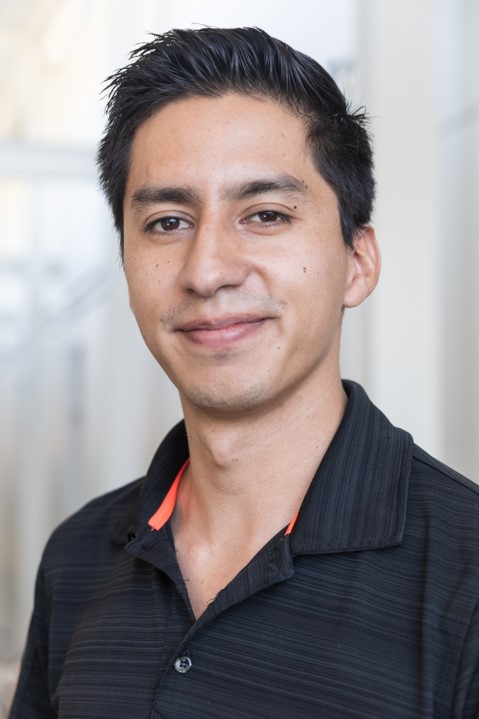
\includegraphics[width=0.8\columnwidth]{photo.jpg}\\[\baselineskip]\end{center} % Your photo
		\small % Smaller font size
		\textbf{José M. Rodríguez-Flores}\\ % Your name
		\color{black}e-mail:\\\url{jrodriguezflores3@ucmerced.edu} \\ % Your email address
		P: (209) 631 2159 \\ % Your phone number
		\Sep % Some whitespace
		\color{black}\textbf{Address} \\
		\color{black}226 W 23rd street\\ % Address 1
		Merced, CA 95340 \\ % Address 2
		USA \\ \vspace{0.2 in}\color{black}\textbf{Twitter}\color{black}\\\url{ @joss__rodriguez}% Address 3
		\\ \vspace{0.2 in}\color{black}\textbf{Website}\color{black}\\\url{josemrodriguezf.github.io}
		\vfill % Whitespace under this block to push it up under the photo
	\end{flushright}
}
%----------------------------------------------------------------------------------------

\begin{document}

\userinformation % Print your information in the left column

\framebreak % End of the first column

%----------------------------------------------------------------------------------------
%	HEADING
%----------------------------------------------------------------------------------------

\cvheading{José Manuel Rodríguez Flores} % Large heading - your name

\cvsubheading{Ph.D Candidate Environmental Systems} % Subheading - your occupation/specialization

%----------------------------------------------------------------------------------------
%	ABOUT ME
%----------------------------------------------------------------------------------------

\aboutme{About Me:}{Agricultural Economist and Ph.D Candidate at University of California Merced in the Environmental Systems program. Specialist in water and agricultural economics. I study coupled human-water systems using optimization and statistical modeling tools to understand the dynamics and feed-backs of this system. I incorporate uncertainty and multi-objective frameworks in my research. Currently working on the agricultural-water system adaptation to climate change and groundwater management policies in California, US.}

%----------------------------------------------------------------------------------------
%	EDUCATION
%----------------------------------------------------------------------------------------

\CVSection{Education}

%------------------------------------------------

\CVItem{2011 - 2015, Universidad Autónoma Chapingo, México}{B.S. in Agricultural Economics}

%------------------------------------------------

\CVItem{2016 - 2018, Colegio de Postgraduados, México}{M.S. in Economics}

%-----------------------------------------------
\CVItem{2019 - present, University of California, Merced}{Ph.D. in Environmental Systems, advanced to candidacy in May 2021}
%------------------------------------------------

\Sep % Extra whitespace after the end of a major section

%----------------------------------------------------------------------------------------
%	EXPERIENCE
%----------------------------------------------------------------------------------------

\CVSection{Experience}

%------------------------------------------------

\CVItem{February - April, 2015. \textit{Research Internship}} {Oklahoma State University, School of Business, Stillwater, OK}


\vspace{0.2 cm}

\CVItem{May - July, 2018. \textit{Research Internship}} {University of California, Merced.}
Project: Insights from a Calibrated Optimization Model for Irrigated Agriculture under Drought in an Irrigation District on the Central Mexican High Plains. Research internship with Professor Dr. Josué Medellín-Azuara\\

\CVItem{2019 - present, \textit{Graduate Student Researcher}}{University of California, Merced.}

Collaboration in projects:
	\begin{itemize}
		\item Hydro-economic analysis of the Sustainable Groundwater Management Act in Kern County, California
		\item Open-DAP: Agricultural Production Model for the Sacramento-San Joaquin Delta
		\item 2020-2021 Drought Economic Impacts in Agriculture in California commissioned by the California Department of Food and Agriculture
	\end{itemize}

Main Tasks: 

\begin{itemize}
	\item Modeling development using Python.
	\item Economic analysis of agriculture and water policy.
\end{itemize}

%------------------------------------------------

%\CVItem{Jan 2008 - Oct 2012, \textit{Computer Repair Specialist}, Buy More}{Worked in the Nerd Herd and helped to solve computer problems by asking customers to turn their computers off and on again.}

%------------------------------------------------

\Sep % Extra whitespace after the end of a major section

%----------------------------------------------------------------------------------------

\clearpage % Start a new page
\userinformation % Print your information in the left column
\framebreak % End of the first column


\CVSection{Publications}

%------------------------------------------------

\CVItem{\textit{Peer-reviewed Journal Articles}}

Fernandez-Bou, Angel Santiago, J. Pablo Ortiz-Partida, Leticia M. Classen-Rodriguez, Chantelise Pells, Kristin B. Dobbin, Vicky Espinoza, \textbf{José Manuel Rodríguez-Flores} et al. "3 Challenges, 3 Errors, and 3 Solutions to Integrate Frontline Communities in Climate Change Policy and Research: Lessons From California." Frontiers in Climate (2021): 104.\\

\textbf{Rodríguez-Flores, José M.}, Jorge A. Valero-Fandiño, Spencer A. Cole, Keyvan Malek, Tina Karimi, Harrison B. Zeff, Patrick M. Reed, Alvar Escriva-Bou, and Josué Medellín-Azuara. "Global Sensitivity Analysis of a Coupled Hydro-Economic Model and Groundwater Restriction Assessment." Pre-print (2020)\\

\textbf{Rodríguez-Flores, José M.}, Josué Medellín-Azuara, Ramón Valdivia-Alcalá, Oscar A. Arana-Coronado, and Roberto C. García-Sánchez. "Insights from a calibrated optimization model for irrigated agriculture under drought in an irrigation district on the central Mexican high plains." Water 11, no. 4 (2019): 858.\\

\CVItem{\textit{Reports}}

Angel Santiago Fernandez-Bou, J. Pablo Ortiz-Partida, Chantelise Pells, Leticia M. Classen-Rodriguez,
Vicky Espinoza, \textbf{Jose M. Rodríguez-Flores}, Lorenzo Booth, Julia Burmistrova, Alan Cai, Ariadna Cairo, John A. Capitman, Spencer Cole, Humberto Flores-Landeros, Alexander Guzman, Mahesh L. Maskey, Dalia Martínez-
Escobar, Pedro Andres Sanchez-Perez, Jorge Valero-Fandiño, Joshua H. Viers, Leroy Westerling, and Josué Medellín-Azuara. 2021. Regional Report for the San Joaquin Valley Region on Impacts of Climate Change. California Natural Resources Agency. Publication number: SUM-CCCA4-2021-003.\\

\CVItem{\textit{Other}}

\textbf{José M. Rodríguez-Flores}, Spencer A. Cole, Alexander Guzman, Josué Medellín-Azuara, Jay R. Lund, Daniel A. Sumner. \textit{Lessons from Three Decades of Evolution of Cropland use in the Central Valley}, California Water Blog, 09/01/2021, \url{https://bit.ly/3qUCFCw}\\

\CVSection{Selected Conferences}

\CVItem{\textit{Conference Posters and Abstracts}}

\textbf{Jose M Rodriguez Flores}, Spencer Cole, Jorge A Alberto Valero Fandino, Keyvan Malek, Tina Karimi, Harrison Bray Zeff, Alvar Escriva-Bou, Josue Medellin-Azuara, Global Sensitivity Analysis for a coupled Hydro-economic model under a groundwater management policy in Kern County, California. AGU Fall Meeting 2020, 2020.\\

Medellin-Azuara, Josue, Alvar Escriva-Bou, \textbf{Jose Rodriguez-Flores}, Jorge Valero-Fandino, and Spencer Cole. "A Multi-Objective Framework for Agricultural Production and Water Use in California's Greater Kern Region under Groundwater Sustainability Regulations." In EGU General Assembly Conference Abstracts, p. 13286. 2020.\\

%------------------------------------------------
%------------------------------------------------

%\Sep % Extra whitespace after the end of a major section

%----------------------------------------------------------------------------------------
%	SKILLS
%----------------------------------------------------------------------------------------
%\Sep % Extra whitespace after the end of a major section

%----------------------------------------------------------------------------------------
%	NEW PAGE DELIMITER
%	Place this block wherever you would like the content of your CV to go onto the next page
%----------------------------------------------------------------------------------------

\clearpage % Start a new page
\userinformation % Print your information in the left column
\framebreak % End of the first column


\CVSection{Software Skills}

%------------------------------------------------

\CVItem{Programming}
{\begin{tabular}{p{0.2\textwidth} p{0.2\textwidth} p{0.2\textwidth}}
\bluebullet Matlab &  \bluebullet R & \bluebullet Python\\
\bluebullet GAMS &  \bluebullet Stata &  \bluebullet LaTex
\end{tabular}}


\CVSection{Service and leadership}

\CVItem{2021-2022, \textit{UC Merced ES Graduate Group}}{Part of the Environmental Systems Seminar Committee \\ \url{https://es.ucmerced.edu/ES-Seminar-Committee}}

\CVSection{Awards}

%------------------------------------------------
\CVItem{2019-present, \textit{Graduate Scholarship for Ph.D studies}}{UC-Mexus-National Science and Technology Council of México}

\CVItem{2016-2018, \textit{Graduate Scholarship for excellence}}{National Science and Technology Council of México.}


\CVItem{2015, \textit{Graduated with honors.}}{Universidad Autonoma Chapingo,Bachelors degree.}


%------------------------------------------------

\Sep % Extra whitespace after the end of a major section

%----------------------------------------------------------------------------------------
%	INTERESTS
%----------------------------------------------------------------------------------------

\CVSection{Interests}

%------------------------------------------------

\CVItem{Professional}{Hydro-economic modeling,  water management, agricultural economics, water governance, socio-hydrology, uncertainty, robust decision making}

%------------------------------------------------

\CVItem{Personal}{Yoga, running, nature and art enthusiast.}

%------------------------------------------------

\Sep % Extra whitespace after the end of a major section

%----------------------------------------------------------------------------------------

\end{document}
